\documentclass{article}
\usepackage[UTF8]{ctex}
\usepackage{geometry}
\usepackage{natbib}
\geometry{left=3.18cm,right=3.18cm,top=2.54cm,bottom=2.54cm}
\usepackage{graphicx}
\pagestyle{plain}	
\usepackage{setspace}
\usepackage{caption2}
\usepackage{float}
\usepackage{datetime} %日期
\renewcommand{\today}{\number\year 年 \number\month 月 \number\day 日}
\renewcommand{\captionlabelfont}{\small}
\renewcommand{\captionfont}{\small}
\begin{document}

\begin{figure}
    \centering
    
\includegraphics[width=8cm]{upc.png}

    \label{figupc}
\end{figure}

	\begin{center}
		\quad \\
		\quad \\
		\heiti \fontsize{45}{17} \quad \quad \quad 
		\vskip 1.5cm
		\heiti \zihao{2} 《计算科学导论》课程总结报告
	\end{center}
	\vskip 2.0cm
		
	\begin{quotation}
% 	\begin{center}
		\doublespacing
		
        \zihao{4}\par\setlength\parindent{7em}
		\quad 

		学生姓名:\underline{\qquad  孙百乐 \qquad \qquad}

		学\hspace{0.61cm} 号:\underline{\qquad 2007010218\qquad}
		
		专业班级:\underline{\qquad 人工智能2001 \qquad  }
		
        学\hspace{0.61cm} 院:\underline{计算机科学与技术学院}
% 	\end{center}
		\vskip 2cm
		\centering
		\begin{table}[h]
            \centering 
            \zihao{4}
            \begin{tabular}{|c|c|c|c|c|c|c|}
            % 这里的rl 与表格对应可以看到,姓名是r,右对齐的;学号是l,左对齐的;若想居中,使用c关键字。
                \hline
                课程认识 & 问题思 考 & 格式规范  & IT工具  & Latex附加  & 总分 & 评阅教师 \\
                30\% & 30\% & 20\% & 20\% & 10\% &  &  \\
                \hline
                 & & & & & &\\
                & & & & & &\\
                \hline
            \end{tabular}
        \end{table}
		\vskip 2cm
		\today
	\end{quotation}

\thispagestyle{empty}
\newpage
\setcounter{page}{1}
% 在这之前是封面,在这之后是正文
\section{引言}
大一上学期,由孙运雷老师为我们讲授了《计算科学导论》这门课。除了讲课外,孙老师还布置了分组演讲任务,课程结束后,我收获不少,现总结如下。

\section{对计算科学导论这门课程的认识、体会}

《计算科学导论》从科学哲学的角度出发,系统地介绍了计算科学的定义,特点,范畴,形态,历史渊源,发展变化,知识组织结构和分类体系,学科专业培养模式和课程体系等内容,有助于学生比较全面的了解计算科学。\par 
研究计算科学,应该是非常难的,但是意义重大。首先可以用于计算机,哪些问题是计算机可以解决的?哪些问题计算机不可能解决?如果计算机可以解决,那么它该如何解决?怎么样让计算机计算问题更快效率更高?其次,计算科学能帮助我们认识自然,如果物理世界是可以计算的,那么我们是否可以通过计算来模拟世界?人类的科学几乎全是建立在计算之上,经验可能会出错,计算会出错吗?这些问题,很值得人类研究。\par 
计算科学导论这门课放在大一,说白了就是为了让刚进入大学的新生对自己大学四年要学的内容有整体认识。但是这本书讲的内容还是比较枯燥难懂的,有很多概念是我们从未见过的,比如什么“计算机语义学”,“图灵机”等等,再加上这本书干货很多,书里概括性的一句话都可能拿出来再写一本书,所以我们理解起来还是很困难的。不过还好,有孙老师为我们讲解这门课,他知识广博,思维跳跃,讲课深入浅出,使我们在对课本内容有了解之外,还能学到其它知识。\par 
上完这个课,当别人问我学计算机是不是就是学修电脑的,我可以很肯定的告诉她我学的不只是修电脑。\par 


\subsection{同学们的分组演讲}
计导课还有一个很重要的部分就是分组演讲,孙老师准备了1500多个课题给同学们选择,很多同学讲的都很有意思。后来演讲改为线上,我也经常参与。\par 
我们班第一组演讲课题是“人流检测”,最开始的人流检测用的是闸机,是纯机械装置,现在依然很常见,在石大图书馆,青岛海洋馆,北京天安门广场我都见到过。现在有了新了选择,比如商场可以用wifi,人脸识别等技术实现无感知地检测人流量。生活中习以为常的东西,我不以为意。但其实每一项技术都有它的发展历史和未来趋势。这启示了我,不要总是想在大的方面取得成就,比如研究深度学习,这太难了。不如把眼光放低,把某项小的技术做到NO.1,也很不错。\par
还有同学演讲题目是指纹识别,虹膜识别等技术。这两种技术其实很早就诞生了,但是指纹识别近几年发展迅速,而虹膜识别确一直不上台面,这是为什么呢?因为指纹识别才是真正的需求。苹果第一个把指纹识别做到了手机上,消费者惊呆了,居然这么好用!这也是苹果的伟大之处,它能做到“生产决定需求”。从此以后,各个厂商纷纷效仿,在手机上加入指纹,指纹技术越来越先进,价格却越来越便宜。现在还有超声波指纹,可以实现屏下指纹识别。虹膜识别本来就有难以攻克的问题,再加上指纹识别已经抢占了全壁江山,现在再去做虹膜识别就是自寻死路。\par 
孙老师说,判断力十分重要,我们要判断什么才是真需求,什么是假需求。判断这个其实不太容易,当年西方人第一次到非洲时,看见非洲人不穿鞋,以为发现了巨大商机。但其实非洲人根本不需要鞋,所以鞋对非洲人来说就是假需求。英国人工业革命后开辟中国市场,往中国卖纺织品,中国是纺织大国,对这玩意也没什么需求,所以英国人卖不出去只能卖鸦片。现在时代变化的这么快,浪潮是一波接一波,有的浪潮很高很大,有的浪潮很小很矮,就是如果我们具有了判断力,就能够勇立潮头,经久不衰。雷军有一个“风口上的猪理论”,很有意思,就是说:如果你站在风口上,即使你是一头猪也能起飞。所以上完课后我知道了判断力是我需要培养的。\par 
还有同学讲到人工智能下围棋,孙老师补充说围棋已经被人工智能玩到顶了,目前来看,人类是不可能在围棋方面打过人工智能了。围棋是一种玩家有全知视角的游戏,现在谷歌的团队在搞能打非全知视角游戏的人工智能,比如说打星际争霸啥的,这样的游戏有战争迷雾,有一定的未知性,有的时候赢了不是靠技术而是靠运气。我觉得这玩意还是挺可怕的,现在电竞那么火,万一这个也被人工智能攻克了,那肯定会触犯到一大波人的利益。所以我觉得这个不是很好的发展方向。\par 
我们现在还处于弱人工智能时代,现在人工智能的局势是:在一些方面能很好代替人,但在绝大多数领域,人工智能在人类眼里还是人工智障,不可能取代人。我觉得现在这个时代还挺好,万一哪天人工智能真发展到有意识的那种,像电影里演的那样早饭把人类干掉了那就完蛋了。\par 

\subsection{对本研班的看法}
我觉得进本研班的一大好处就是避免了“卷”的风气。我观察到,在其它班级里会有同学还保持高中的思维,对成绩有一种执念。有的人在寝室里展现出自己不学习的样子,然后在自习室里“偷学”。一口一个“大佬”称呼别人,实际上心里非常害怕别人超过自己。这样的人,继承了高中的传统,仍然觉得成绩最重要。同时又目光短浅,不立志考全校第一,只求比寝室里的同学考得好就行。这也是正常现象,毕竟其它班级有考研,保研的压力。这样的好处是:保持了积极的学习态度,至少比那些刚进入大学就堕落的人强。坏处就是:进入大学之后并没有明确的目标,不知道自己真正想要干什么,就只能在成绩上较劲。\par 
本研班没有争保研名额的压力,所以有一部分同学貌似在混日子,没看出来他想干什么。好处是大家都相处的很融洽,没有任何“窝里斗”的迹象。大家都在寻找自己感兴趣的事做,有的人喜欢智能车,有的人喜欢打acm,有的人喜欢打篮球,甚至他已经在学校里当裁判了。如果大家都能有自己的想法,尽早投身到自己喜欢的领域,就更有可能做出更大的成就来。我挺喜欢本研班的,我理想中的班级氛围应该是:上课的时候大家一起认真学习,打好数理基础。下课时分成若干个小组去做一些实践项目,在实践中学习一些课堂学不到的东西。我呆在这个班级里,我希望我身边能多一些积极上进的人,我们一起搞大事情。\par 
孟子说,穷则独善其身,达则兼济天下。我现在有的是时间和精力,我想以我的方式多参与到班级事务当中,协助班长一起营造良好的班级氛围。我很喜欢何为班长,他在当班长方面,可以说算是一个“专家”,是有天分的,值得我信赖,我也能从他身上学到东西。孙老师也说要多管“闲事”,在参与班级事务的过程中我也能培养我的管理和人际交往能力。不过我这个年龄的人,思想还很幼稚,做事情是摸着石头过河,走一步算一步。不过没关系,我会敢于试错,正如屈原所说,路漫漫其修远兮,吾将上下而求索。\par 

\section{进一步的思考}
\subsection{图像识别的历史}
1966年的夏天,人工智能之父Minsky给学生布置了一个暑假作业。要求学生通过编写一个程序,让计算机告诉我们它通过摄像头看到了什么。\par 
1970s~1980s:代电子计算机的出现,让计算机有机会尝试回答出它看到了什么东西。研究人员首先从人类看东西的方法中获得借鉴。当时人们普遍认为,人类能看到并理解事物是因为通过两只眼睛可以立体地观察事物(现在看来当然是极大的误解……)。因此要想让计算机理解它所看到的图像,必须先将事物的三维结构从二维的图像中恢复出来,这就是所谓的“三维重构”的方法。\par 
另一个灵感是,人们认为人之所以能识别出一个苹果,是因为人们已经有了先验知识:苹果是红色的、圆的、表面光滑的。如果给机器也建立一个这样的知识库,让机器将看到的图像与之匹配,是否可以让机器识别乃至理解它所看到的东西呢,这是所谓的“先验知识库”的方法。\par 
这套方法只能够提取少数基本特征,实用性当然不高,只能用在某些光学字符识别、工件识别、显微/航空图片的识别等。\par 
1990s:到了上世纪九十年代,图像处理硬件技术有了飞速进步,人们也开始尝试不同的算法,包括统计方法和局部特征描述符的引入,使得计算机视觉技术取得了更大的发展,并开始广泛应用于工业领域。在“先验知识库”的方法中,事物的形状、颜色、表面纹理等特征受到视角和观察环境所影响,在不同角度、不同光线、不同遮挡的情况下会产生变化。因此,研究者的新方法是,通过局部特征的识别来判断事物,对事物建立一个局部特征索引,即使视角或观察环境发生变化,也能比较准确地匹配上。\par 
2000s:进入21世纪,得益于互联网兴起和数码相机出现带来的海量数据,加之机器学习方法的广泛应用,计算机视觉发展迅速。以往许多基于规则的处理方式,都被机器学习所替代:机器自动从海量数据中总结归纳物体的特征,然后进行识别和判断。这一阶段涌现出了非常多的应用,包括典型的相机人脸检测、安防人脸识别、车牌识别等等。数据的积累还诞生了许多评测数据集,比如权威的人脸识别和人脸比对识别的平台——FDDB和LFW等,其中最有影响力的是ImageNet,包含1400万张已标注的图片,划分在上万个类别里。\par 
2010年以后:到了2010年以后,借助于深度学习的力量,计算机视觉技术得到了爆发增长和产业化。出现了神经网络图像识别,这就是目前比较新的一种图像识别技术了。\par 
\subsection{卷积神经网络}
深度学习是图像识别最新进展的驱动力,智慧教学、视频监控、自动驾驶和智能医疗等有价值的应用正在我们身边发生。深度学习的成功主要得益于三个方面:大规模数据集的生成、强有力的模型的发展和可用的大量计算资源。对于各种图像识别任务,精心设计的深层神经网络已经远远超过了以往基于人工设计图像特征的方法。\par 
\begin{figure}[H]
	\centering
	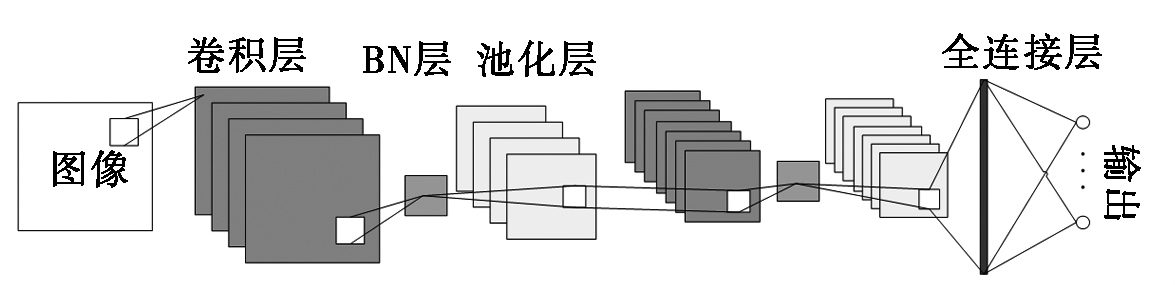
\includegraphics[width=0.7\linewidth]{卷积神经网络}
	\caption{}
	\label{fig:}
\end{figure}
如图是一个简单的卷积神经网络模型。第一层是输入层,输入的图像直接输入到输入层。第二层 是 BN 层,它主要是对卷积层提取到的特征进行归 一化处理。可以改善流经网络的梯度,允许更大的 学习率以及大幅提高模型的训练速度。第三层是池 化层,它计算输入要素图的局部平均值或最大值,主要作用是进行特征降维,压缩数据和参数的数量,减小过拟合,同时提高模型的容错性。接下来的卷积 层,BN 层和池化层以相同的方式运行。最后输出 层是全连接层,输出神经元的最大值是最终分类器 的结果。在演讲的PPT中我放入了几张动图可以更好地展示简单的神经网络在图像识别中的作用。\par 
\subsection{图像识别技术发展中的挑战}

\subsubsection{如何提高模型的泛化能力} 
在图像识别技术得到广泛应用之前,一个重要的挑战是如何知道一个模型对于一个从未见过的场景仍然具有良好的泛化能力。\par 
在目前的实践中,将数据集随机分为训练集和测试集,并在此数据集上对模型进行相应的训练和评估。需要注意的是,在这种方法中,测试集与训练集具有相同的数据分布,因为它们是从具有相似场景内容和成像条件的数据中采样的。\par 
然而,在实践中,测试图像可能来自与训练期间不同的数据分布。这些先前未知的数据可能与训练数据在透视图、大小、场景配置、相机属性等方面有所不同。\par 
一项研究表明,这种数据分布的差异会导致各种深网络模型的精度显著降低。在诸如自动驾驶等关键应用中,当前模型对数据分布的自然变化的敏感性可能成为一个严重的问题。\par 
\subsubsection{自动化网络设计} 
近年来,图像识别这一领域的重心从设计更好的特征转向了设计更新的网络架构。然而,设计网络架构是一个冗长乏味的过程,它需要处理大量的超参数和设计选择。调优这些元素需要有经验的工程师花费大量的时间和精力。更重要的是,一个任务的最优架构和另一个任务的最优架构可能是完全不同的。尽管我们对自动神经架构搜索的研究已经开始了,但它们仍然处于早期阶段并且仅适用于图像分类任务。当前方法的搜索空间非常狭窄,因为它们寻找的是现有网络模块的局部最优组合(例如深度可分离卷积和恒等连接),并且无法发现新的模块。目前还不清楚这些现有的方法是否足以胜任更复杂的任务。
\subsubsection{可解释性问题}
理解和解释深度学习模型是一个比较有挑战的事情,因为大规模训练的深度卷积网络被认为是黑盒系统,也许我们可以对训练的数据集和损失函数有一定的了解,但是对深度模型的学习过程以及生成的预测的理解确实很有限。自然深度学习中的很重要领域人脸识别的可解释性也是一个很大的挑战,当前在这方面探索的方法有网络注意力、网络解剖或综合语言解释,然而,缺乏网络比较和量化可解释结果的真相,尤其是在人脸识别中近亲或近亲之间的差异很微妙,解释并不明显。
\subsubsection{广度优先?深度优先?}
虽然深度学习通过利用大量注释数据在各种任务中取得了巨大的成功,但现有技术经常在小数据场景中崩溃,因为只有少量标记实例可用。这种情况通常被称为“少样本学习”,需要在实践中仔细考虑。例如,一个家庭机器人被期望在它能够向它展示一次新物体就能够认识这个物体。一个人可以自然地完成这项任务,即使这个物体后来被操纵,比如折叠起来的毯子。如何赋予神经网络以人类的泛化能力是一个开放研究的问题。另一个极端是如何利用超大规模数据有效地提高识别算法的性能。对于自主驾驶等关键应用,图像识别的出错代价非常高。因此,研究人员创建了大量的数据集,其中包含了数亿个带有标注丰富的图像,他们希望利用这些数据集使模型更加精确。然而,目前的算法不能很好地利用这样的超大数据量。在包含3亿个带注释图像的JFT数据集上,随着训练数据量的增加,各种深度网络的性能只呈现对数级的提高。在大规模数据的情况下,增加训练数据的效益将越来越不明显,这是一个需要解决的重要问题。
\section{总结}
这门课虽然没怎么听懂,但并不代表我没有从这门课中学到知识。我的收获主要是拓宽了视野,孙老师在课堂上丰富的拓展以及同学们的演讲都让我印象深刻。我应该是我们班在线上听演讲最多的人,我发现大多数同学都和我一样,对很多先进的技术感兴趣,但是了解的确很浅薄,找资料调研的能力也很差,这是以后6年需要提升的。\par 


\section{附录}
\begin{itemize}
    \item 申请Github账户,给出个人网址和个人网站截图
    \item 注册观察者、学习强国、哔哩哔哩APP,给出对应的截图
    \item 注册CSDN、博客园账户,给出个人网址和个人网站截图
    \item 注册小木虫账户,给出个人网址和个人网站截图
\end{itemize}

\begin{figure}[H]
	\centering
	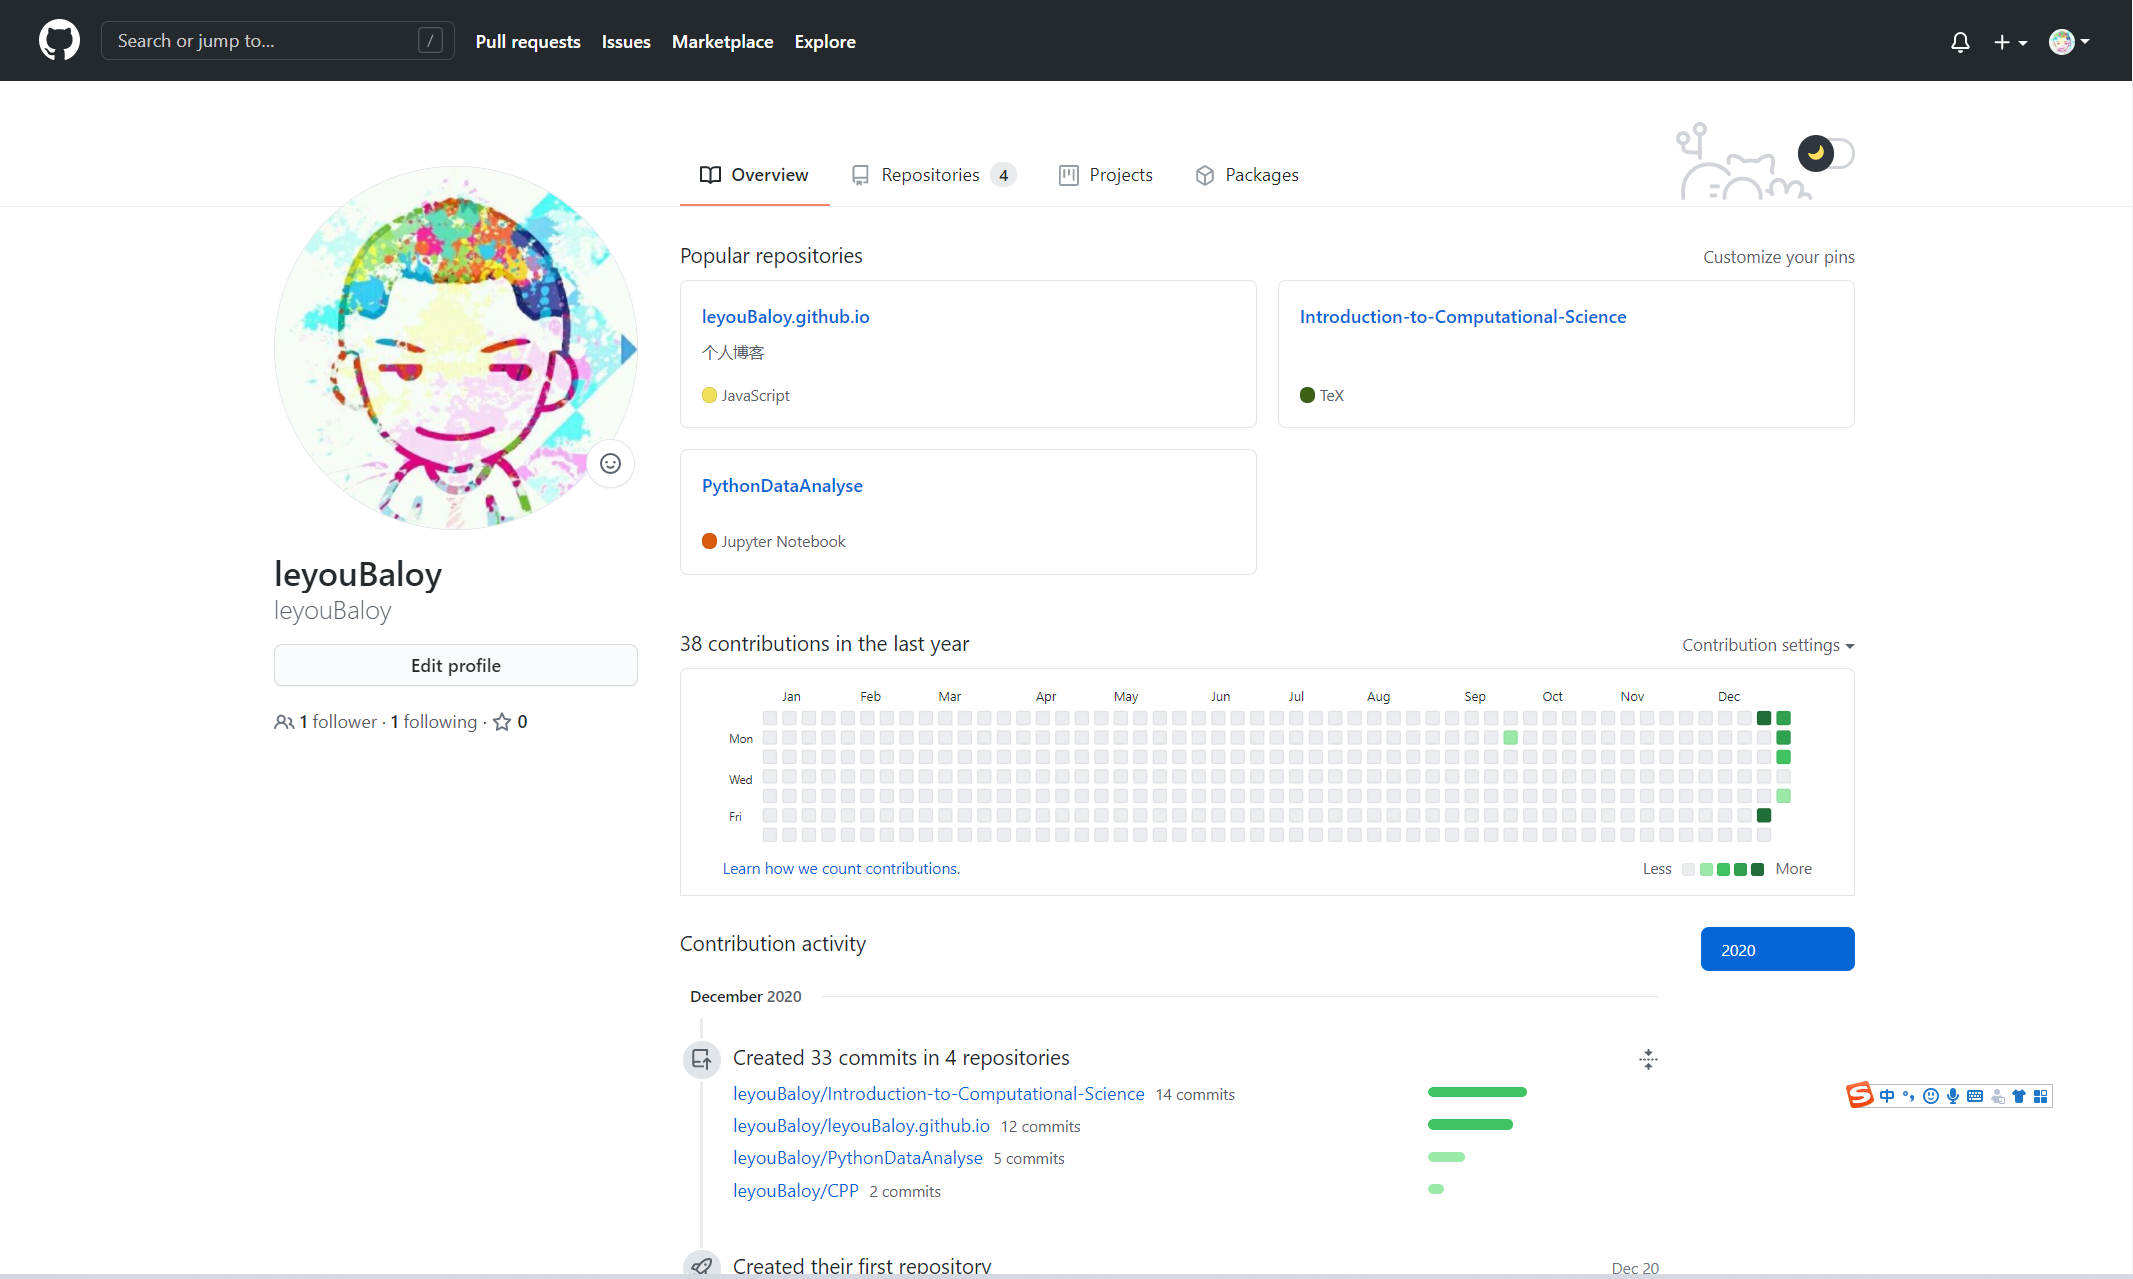
\includegraphics[width=0.7\linewidth]{github}
	\caption{}
	\label{fig:github}
\end{figure}
github个人地址:https://github.com/leyouBaloy \par 
个人博客: http://www.leyoubaloy.xyz/

\begin{figure}[H]
	\centering
	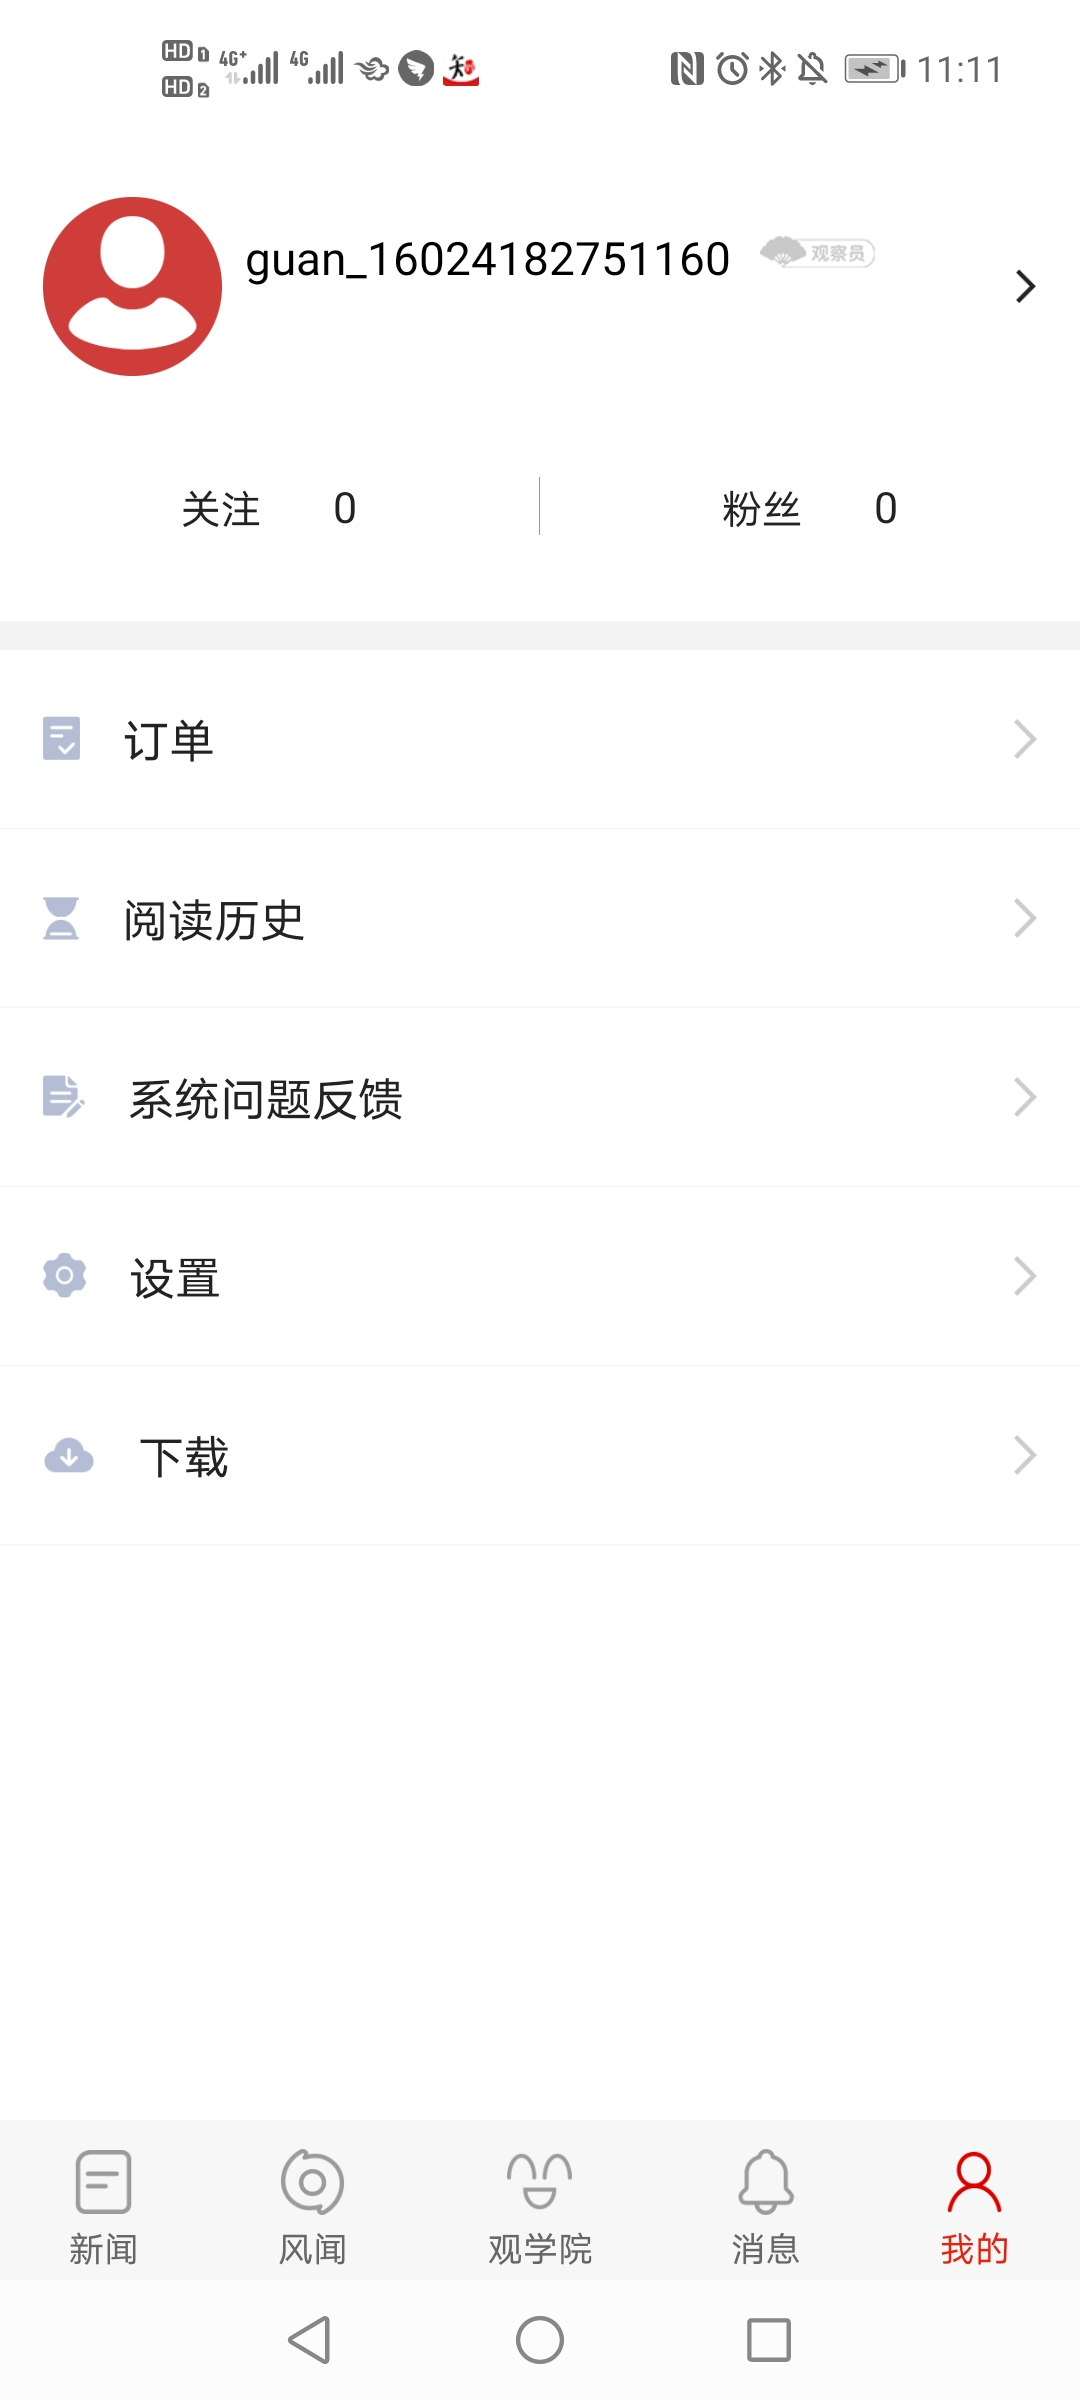
\includegraphics[width=0.3\linewidth]{观察者}
	\caption{}
	\label{fig:}
\end{figure}

\begin{figure}[H]
	\centering
	
\includegraphics[width=0.3\linewidth]{学习强国}
	\caption{}
	\label{fig:}
\end{figure}

\begin{figure}[H]
	\centering
	
\includegraphics[width=0.3\linewidth]{哔哩哔哩}
	\caption{}
	\label{fig:}
\end{figure}

\begin{figure}[H]
	\centering
	
\includegraphics[width=0.3\linewidth]{csdn}
	\caption{}
	\label{fig:csdn}
\end{figure}

\begin{figure}[H]
	\centering
	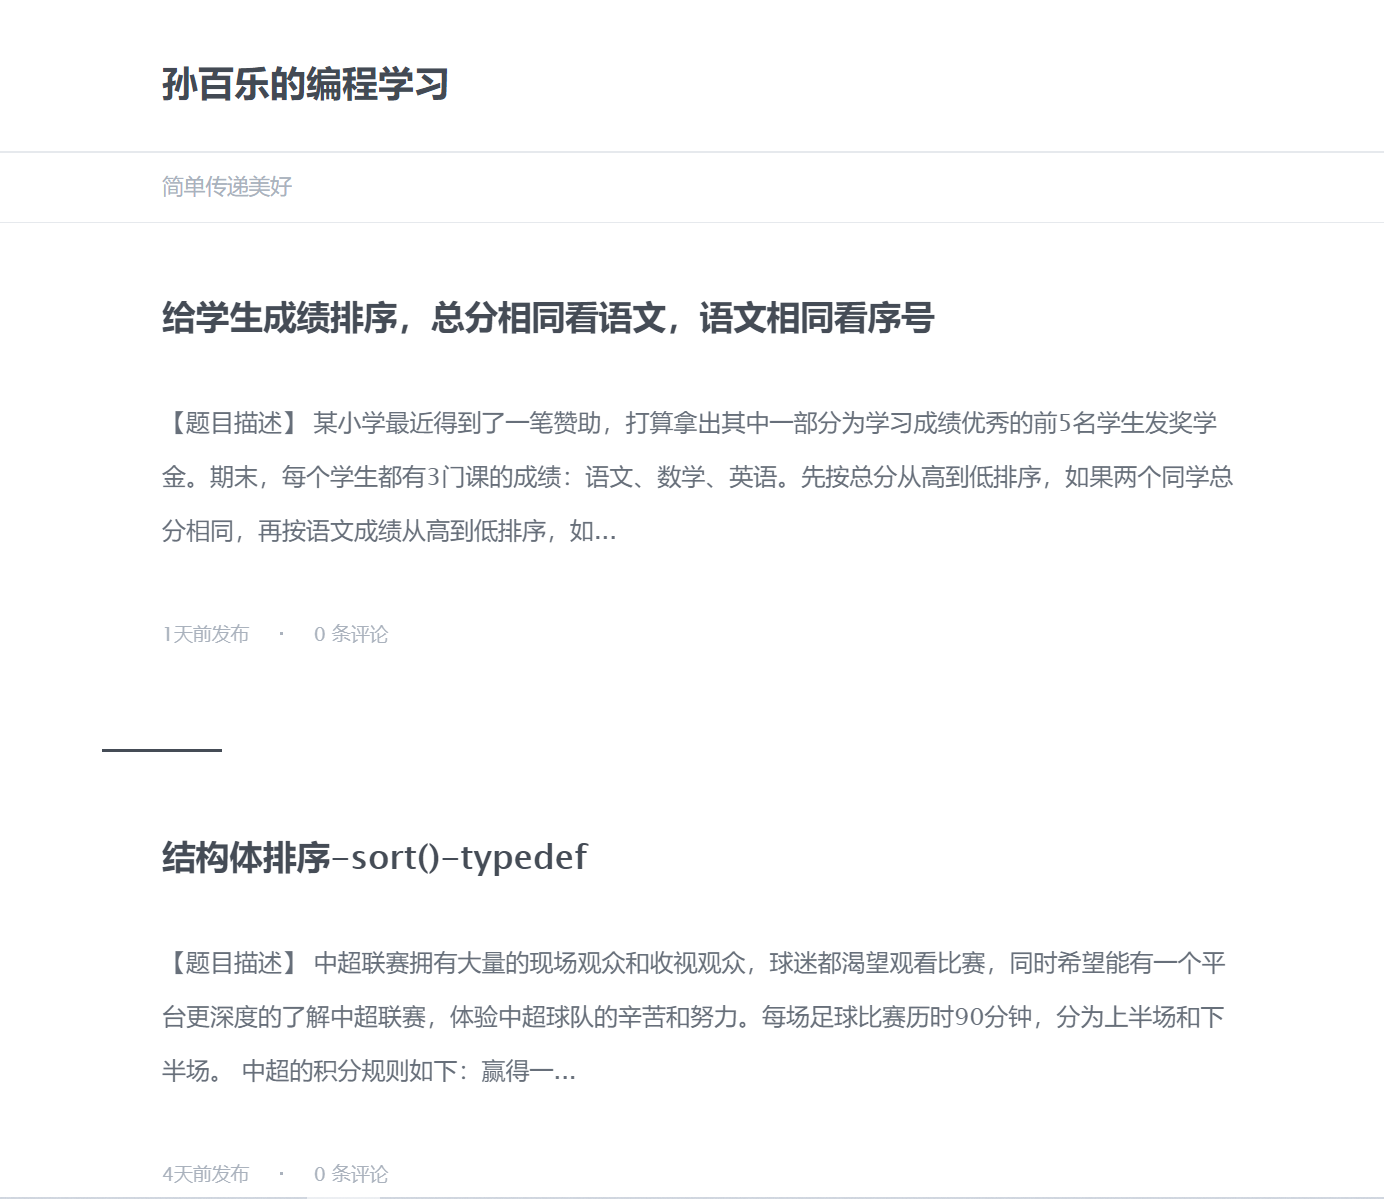
\includegraphics[width=0.7\linewidth]{个人博客}
	\caption{}
	\label{fig:}
\end{figure}
\begin{figure}[H]
	\centering
	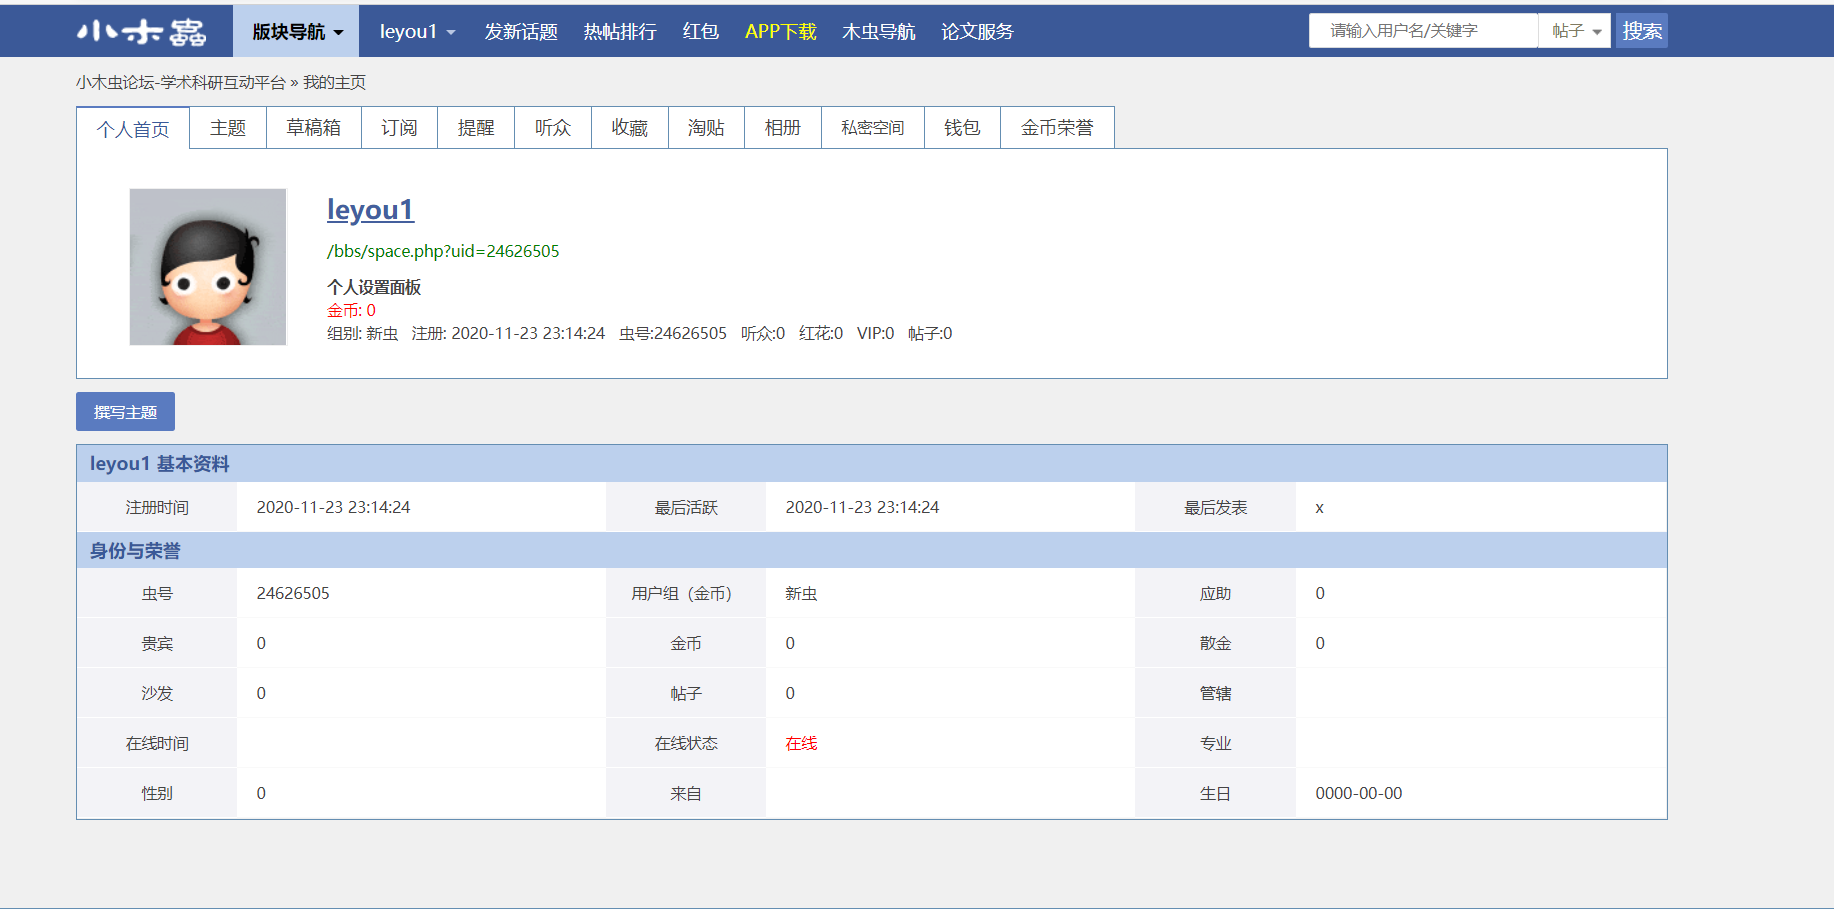
\includegraphics[width=0.7\linewidth]{小木虫}
	\caption{}
	\label{fig:}
\end{figure}


\end{document}
